\chapterimage{head2.png} % Chapter heading image
\chapter{Spectral Finite Element Method}
\section{Domain of sFEM}
The grid size is 0.6250 Å. (The distance between two red points). Totally, there are 193 points.
\begin{center}
        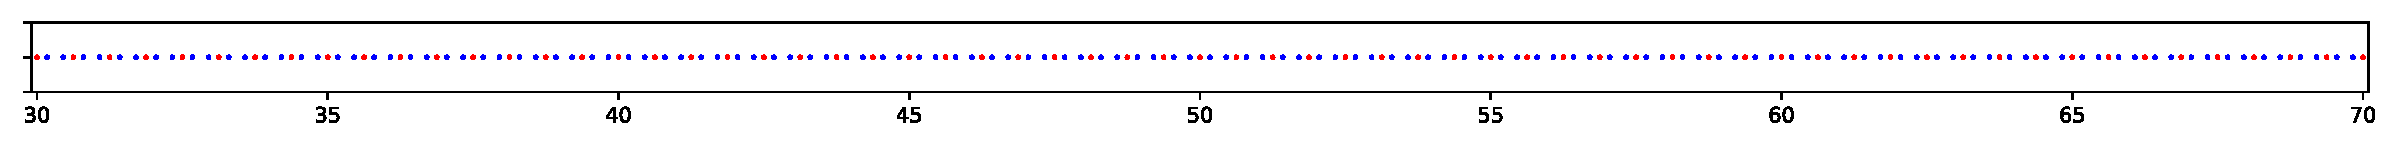
\includegraphics[scale=0.3]{ch3/node.pdf}
\end{center}
\begin{itemize}
        \item The number of spectral element, $N_h=64$
        \item The order of interpolation polynomial, $N_p=4$
\end{itemize}
Therefore, we now have $V$, a vector space  of dimension $193$. This vector space has a natural basis, or we called it the standard basis
\begin{equation}
        \{\textbf{e}_1, \textbf{e}_2, ..., \textbf{e}_{193}\}
\end{equation}
where
\begin{equation}
\textbf{e}_1=  \begin{bmatrix} 1 \\ 0 \\ \vdots \\ 0 \end{bmatrix}~~
\textbf{e}_2=  \begin{bmatrix} 0 \\ 1 \\ \vdots \\ 0 \end{bmatrix}~~
\cdots ~~
\textbf{e}_{193} = \begin{bmatrix} 0 \\ 0 \\ \vdots \\ 1 \end{bmatrix} 
\end{equation}

\begin{definition}[Orthonormal basis from sFEM]
After doing spectral finite element method, we can get a set of orthonormal basis
\begin{equation}
        B = \{ \psi_1, \psi_2, \psi_3, ..., \psi_{72} \}    
\end{equation}
\end{definition}

\begin{definition}[$\rho$ with respect to the $B$ basis]
Now, we have an orthonormal basis $B$, so $\rho$ can be represented
\begin{align*}
        \rho = c_1 \psi_1 + c_2 \psi_2 + \cdots + c_{72} \psi_{72}        
\end{align*}
More precisely,
\begin{align*}
        [\rho]_{B} =  \begin{bmatrix} c_1 \\ c_2 \\ \vdots \\ c_{72} \end{bmatrix}
\end{align*}      
\end{definition}

\section{Weight function, orthogonality and norm}
\begin{definition}[inner product]
By using integral calculus, it is common to use the following to define the inner product of two functions $f$ and $g$ with respect to a nonnegative weight function $w$ over an interval $[a, b]$:
\begin{equation}
        \langle f, g\rangle_w = \int_a^b f(x)g(x)w(x)\,dx \approx \sum_{i=1}^{193}w(x_i)f(x_i)g(x_i) 
\end{equation}
\end{definition}

\begin{definition}[weight function $w(x)$]
From the  Gauss-Lobatto quadrature, we have
\begin{center}
        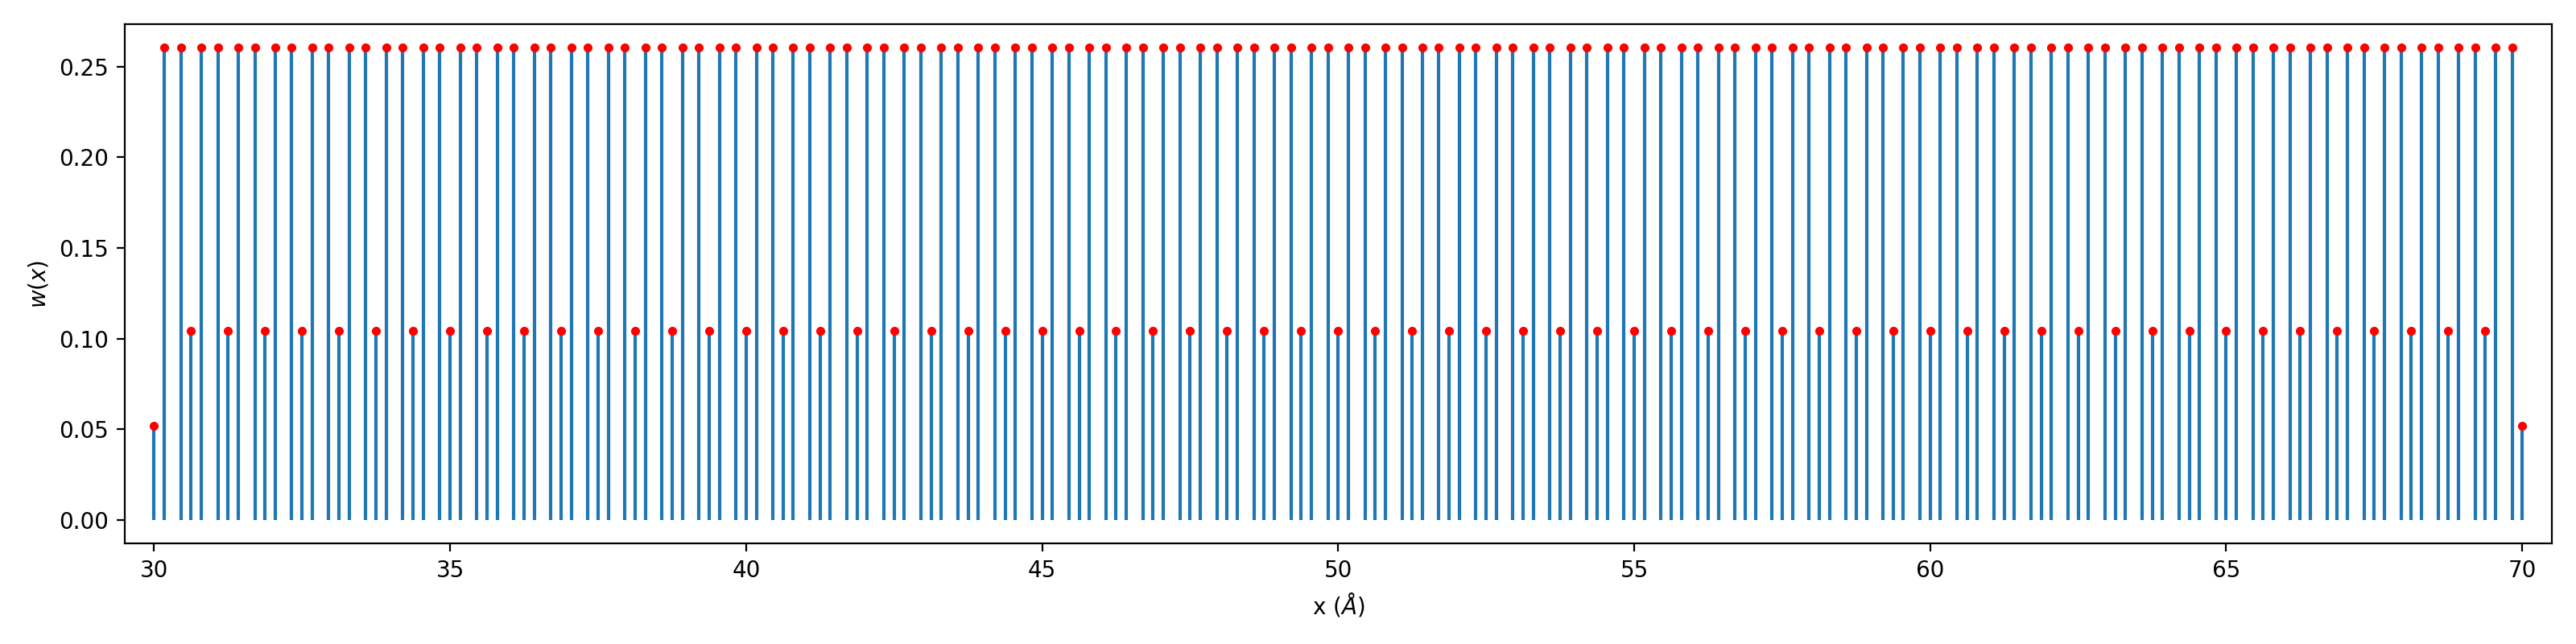
\includegraphics[scale=0.35]{ch3/weight_function.png}   
\end{center}
\end{definition}

\begin{definition}[Orthogonal]
We say that functions $f$ and $g$ are orthogonal if their inner product (equivalently, the value of this integral) is zero:
\begin{equation}
        \langle f,g\rangle _{w}=0.
\end{equation}
\end{definition}

\begin{definition}[Norm]
We define the norm with respect to this inner product as
\begin{equation}
        \|f\|_w = \sqrt{\langle f, f\rangle_w}
\end{equation}
\end{definition}

\section{Diagonalization of the operator}
\begin{definition}[Basis functions]
\begin{align}
        \psi^0_i(x) &= \rho_{\rm eq}(x) \phi^0_i(x) \\
        \phi^0_i(x) &= \sum_n c^0_n u_n(x).
\end{align}
\label{basisfunctions}
\end{definition}

\begin{definition}[Eigenvector matrix]
\begin{equation}
\Psi=
\begin{bmatrix}
\vert & \vert &  & \vert \\
\psi_1(x) & \psi_2(x) & \cdots & \psi_{N_v}(x) \\
\vert & \vert &  & \vert 
\end{bmatrix}
\end{equation}
\label{eigenvectormatrix}
Here, we get a set of orthonormal basis, $\langle \psi_i |$. The left part in the following part is 
\begin{equation}
        \Psi^T_{72\times 193}\Psi_{193 \times 72} = (\Psi^T\Psi)_{72 \times 72}
\end{equation}
The completeness relationship is actually can be seen by the blue points in the right part:
\begin{equation}
        \langle \psi_i(x),\psi_i(x)\rangle _{w} = \sum_{j=1}^{193}w(x_j)\psi_i(x_j)\psi_i(x_j)  = 1
\end{equation}
\begin{center}
        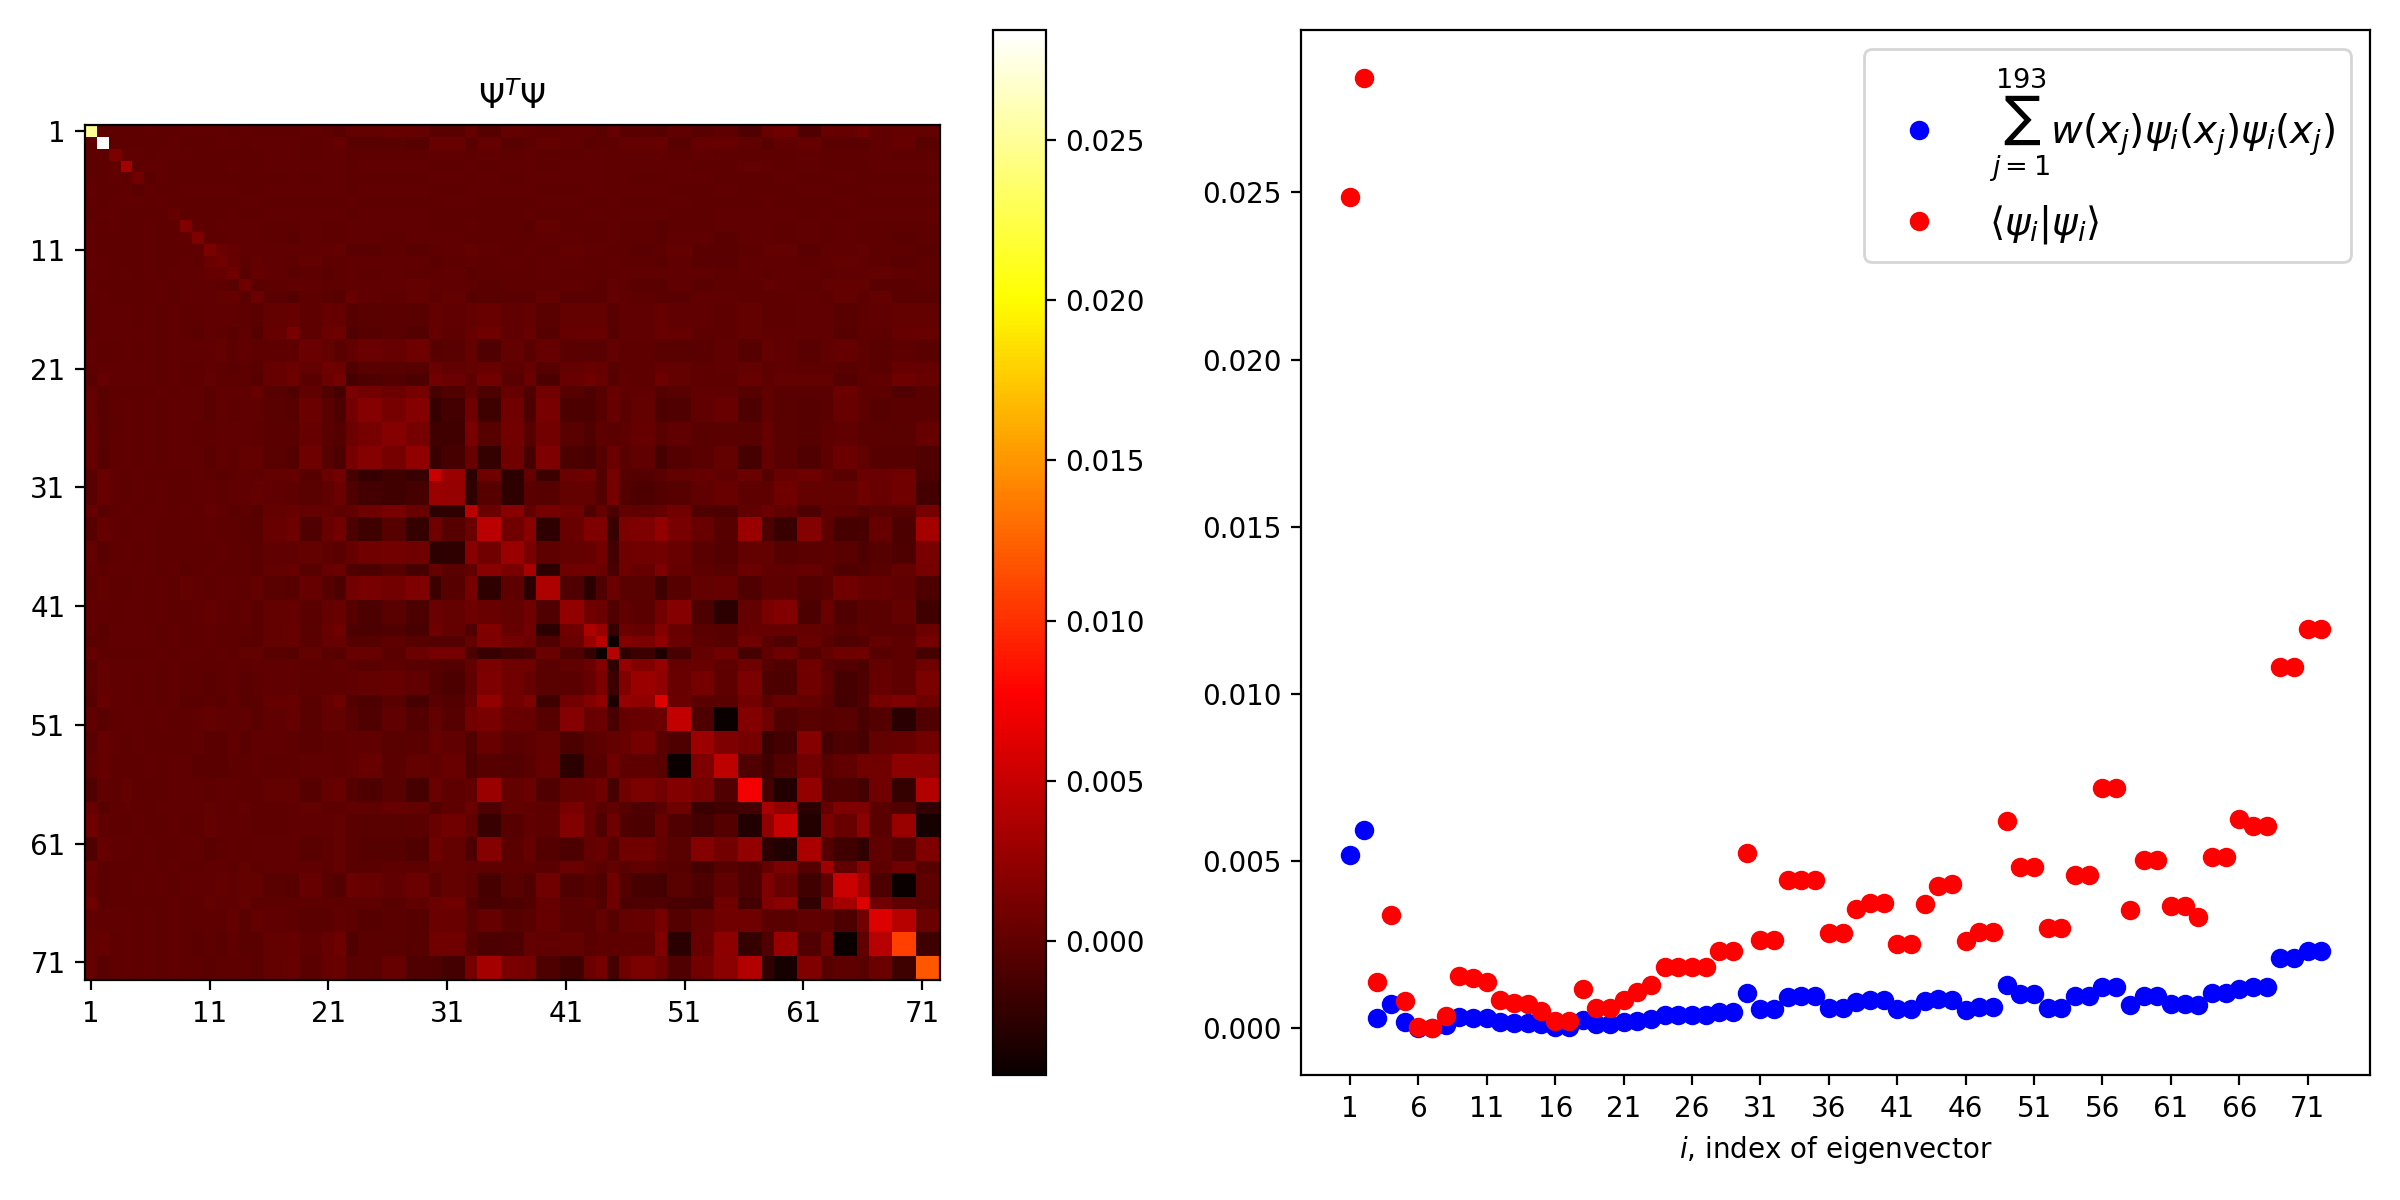
\includegraphics[scale=0.4]{ch3/eigenvec_matrix_complete.png}   
\end{center}
\end{definition}

\section{Photon operator and Emission probability}
Assume we have the graphical model like the following						
\begin{center}
        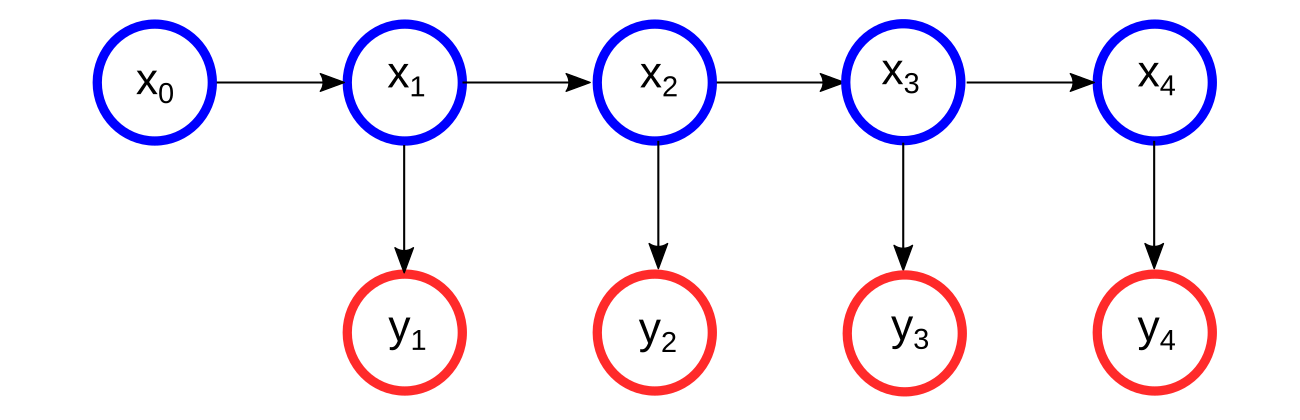
\includegraphics[scale=0.8]{ch2/four_states_ex.png}   
\end{center}
The complete likelihood function is
\begin{equation}
\mathcal{P}(X(t), Y(t)) = p(x_{t_0}) \prod_{\tau=1}^4 p(y_{t_{\tau}}|x_{t_{\tau}}) p(x_{t_{\tau}}|x_{t_{\tau -1}})            
\end{equation}
where the emission probability $p(y_{t_{\tau}}|x_{t_{\tau}})$ is defined by a Gaussian
\begin{equation}
        p(y_{t_{\tau}}|x_{t_{\tau}}) =  \mathcal{N}(\mu = y_{t_{\tau}}  ,\sigma ^{2})       
\end{equation}

\begin{definition}[Emission Probability as linear transformation $T$]
For example, if we have an observation $y_1$ in $t_{1}$, we will propagate like the following:
\begin{align*}
        T(\rho) = \textbf{y} \rho = 
        \begin{bmatrix} 
              f(x_1) & 0 & 0 & \cdots & 0 \\
              0 & f(x_2) & 0 & \cdots & 0 \\
              \vdots & \vdots & \vdots & \vdots & \vdots \\
              0 & 0 & 0 & \cdots & f(x_{193}) \\
        \end{bmatrix}
        \begin{bmatrix} \rho_1 \\ \rho_2 \\ \vdots \\ \rho_{193} \end{bmatrix}    
\end{align*}
We redefine a function $f(x)$ for emission probability
\begin{align*}
f(x; \mu = y_1, \sigma) ={\frac {1}{\sigma {\sqrt {2\pi }}}}e^{-{\frac {1}{2}}\left({\frac {x-\mu }{\sigma }}\right)^{2}}      
\end{align*}
\begin{center}
        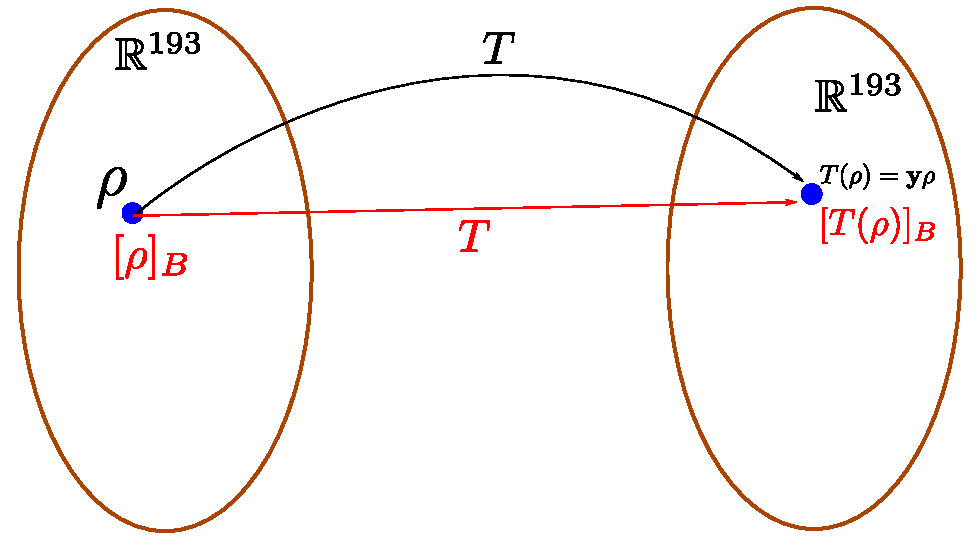
\includegraphics[scale=0.5]{ch3/linear_transform.pdf}   
\end{center}
\end{definition}

\begin{definition}[Transformation matrix with respect to the $B$ basis]
First, the change of basis matrix for $B$
\begin{align*}
        C = 
        \begin{bmatrix}
              \vert & \vert &  & \vert \\
              \psi_1   & \psi_2 & \cdots & \psi_{72} \\
              \vert & \vert &  & \vert
        \end{bmatrix}_{193 \times 72}  
\end{align*}
And its transpose is
\begin{align*}
        C^{T} = 
        \begin{bmatrix}
        - & \psi_1 & - \\
        - & \psi_2 & - \\
         & \vdots & \\
         - & \psi_{72} & - \\
        \end{bmatrix}_{72 \times 193}
\end{align*}
And you can see
\begin{align*}
        C^{T}C = I  
\end{align*}
so \( C^{T}\) is left inverse
\begin{align*}
        C^{T} = C^{-1}  
\end{align*}
\begin{center}
        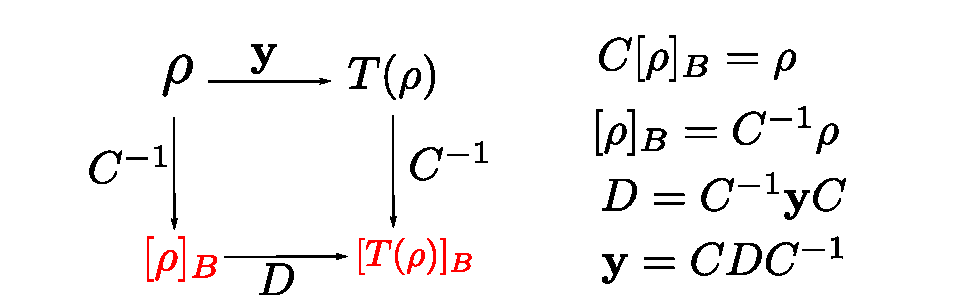
\includegraphics[scale=0.5]{ch3/transform_map.pdf}   
\end{center}
Therefore, we get a transformation matrix $D$ with repect to $B$ basis
\begin{equation}
        [T(\rho)]_{B} = D [\rho]_{B}  
\end{equation}
where
\begin{align*}
        D =  \begin{bmatrix}
                - & \psi_1 & - \\
                - & \psi_2 & - \\
                 & \vdots & \\
                 - & \psi_{72} & - \\
             \end{bmatrix}_{72 \times 193}
          \begin{bmatrix} 
          f(x_1) & 0 & \cdots & 0 \\
          0 & f(x_2) & \cdots & 0 \\
          \vdots & \vdots & \vdots & \vdots \\
          0 & 0 & \cdots & f(x_{193}) \\
          \end{bmatrix}_{193 \times 193}
          \begin{bmatrix}
                \vert & & \vert \\
                \psi_1   & \cdots & \psi_{72} \\
                \vert &  & \vert
          \end{bmatrix}_{193 \times 72}    
\end{align*}
$D$ can also be expressed by bra-ket notation
\begin{align*}
        D=\begin{bmatrix}
                \left< \psi_1(x) | \textbf{y} | \psi_1(x) \right> & \left< \psi_1(x) | \textbf{y} | \psi_2(x) \right> & \cdots & \left< \psi_1(x) | \textbf{y} | \psi_{72}(x) \right> \\
                \left< \psi_2(x) | \textbf{y} | \psi_1(x) \right> & \left< \psi_2(x) | \textbf{y} | \psi_2(x) \right> & \cdots & \left< \psi_2(x) | \textbf{y} | \psi_{72}(x) \right> \\
                \vdots & \vdots & \cdots & \vdots \\
                \left< \psi_{72}(x) | \textbf{y} | \psi_1(x) \right> & \left< \psi_{72}(x) | \textbf{y} | \psi_2(x) \right> & \cdots & \left< \psi_{72}(x) | \textbf{y} | \psi_{72}(x) \right> \\
                \end{bmatrix}_{72 \times 72}
\end{align*}
where
\begin{align*}
        \left< \psi_i(x) | \textbf{y} | \psi_j(x) \right> = \int w(x) \psi_i(x) f(x) \psi_j(x) dx \approx \sum_{k=1}^{193} w(x_k) \psi_i(x_k) f(x_k) \psi_j(x_k)
\end{align*}
\end{definition}

\section{Single Well}
\begin{center}
        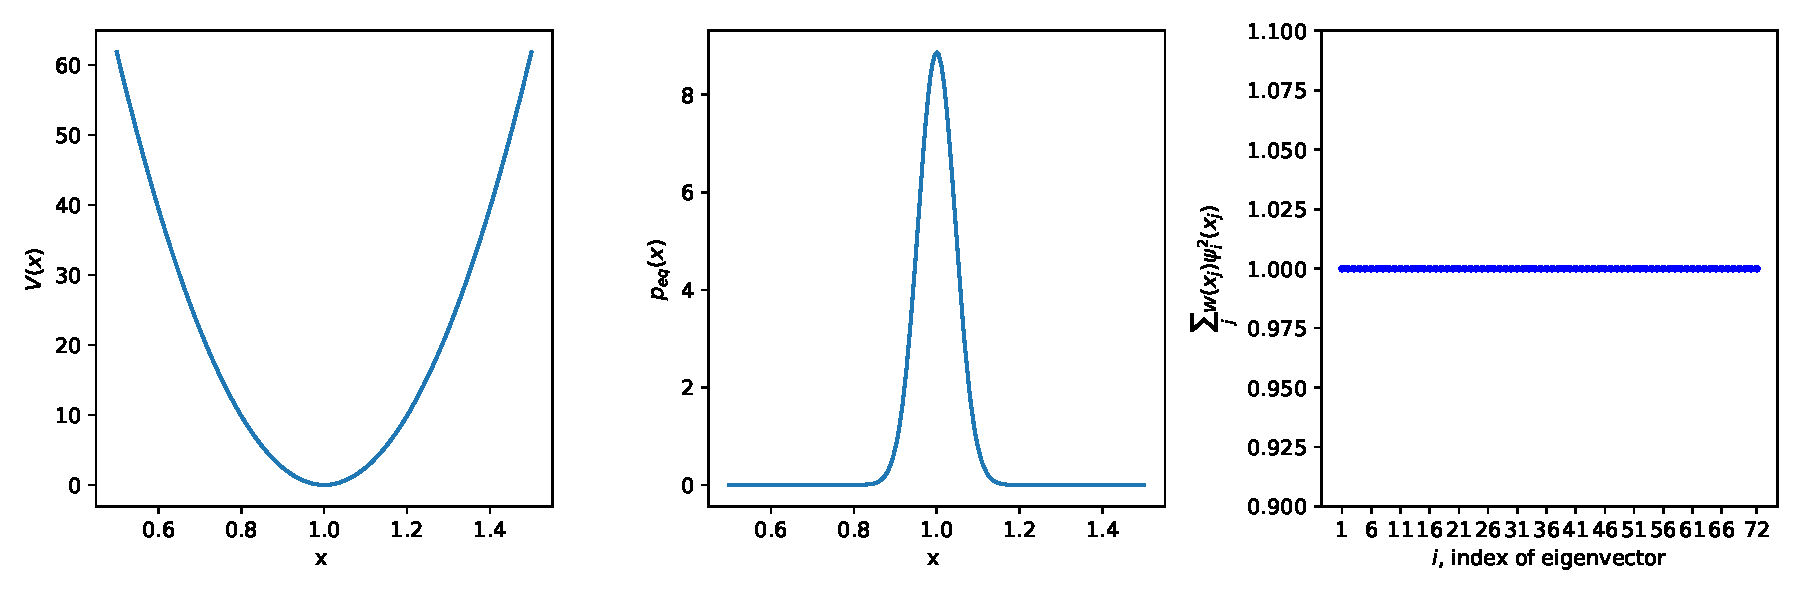
\includegraphics[scale=0.45]{ch3/single_well_1.pdf}   
\end{center}
\begin{center}
        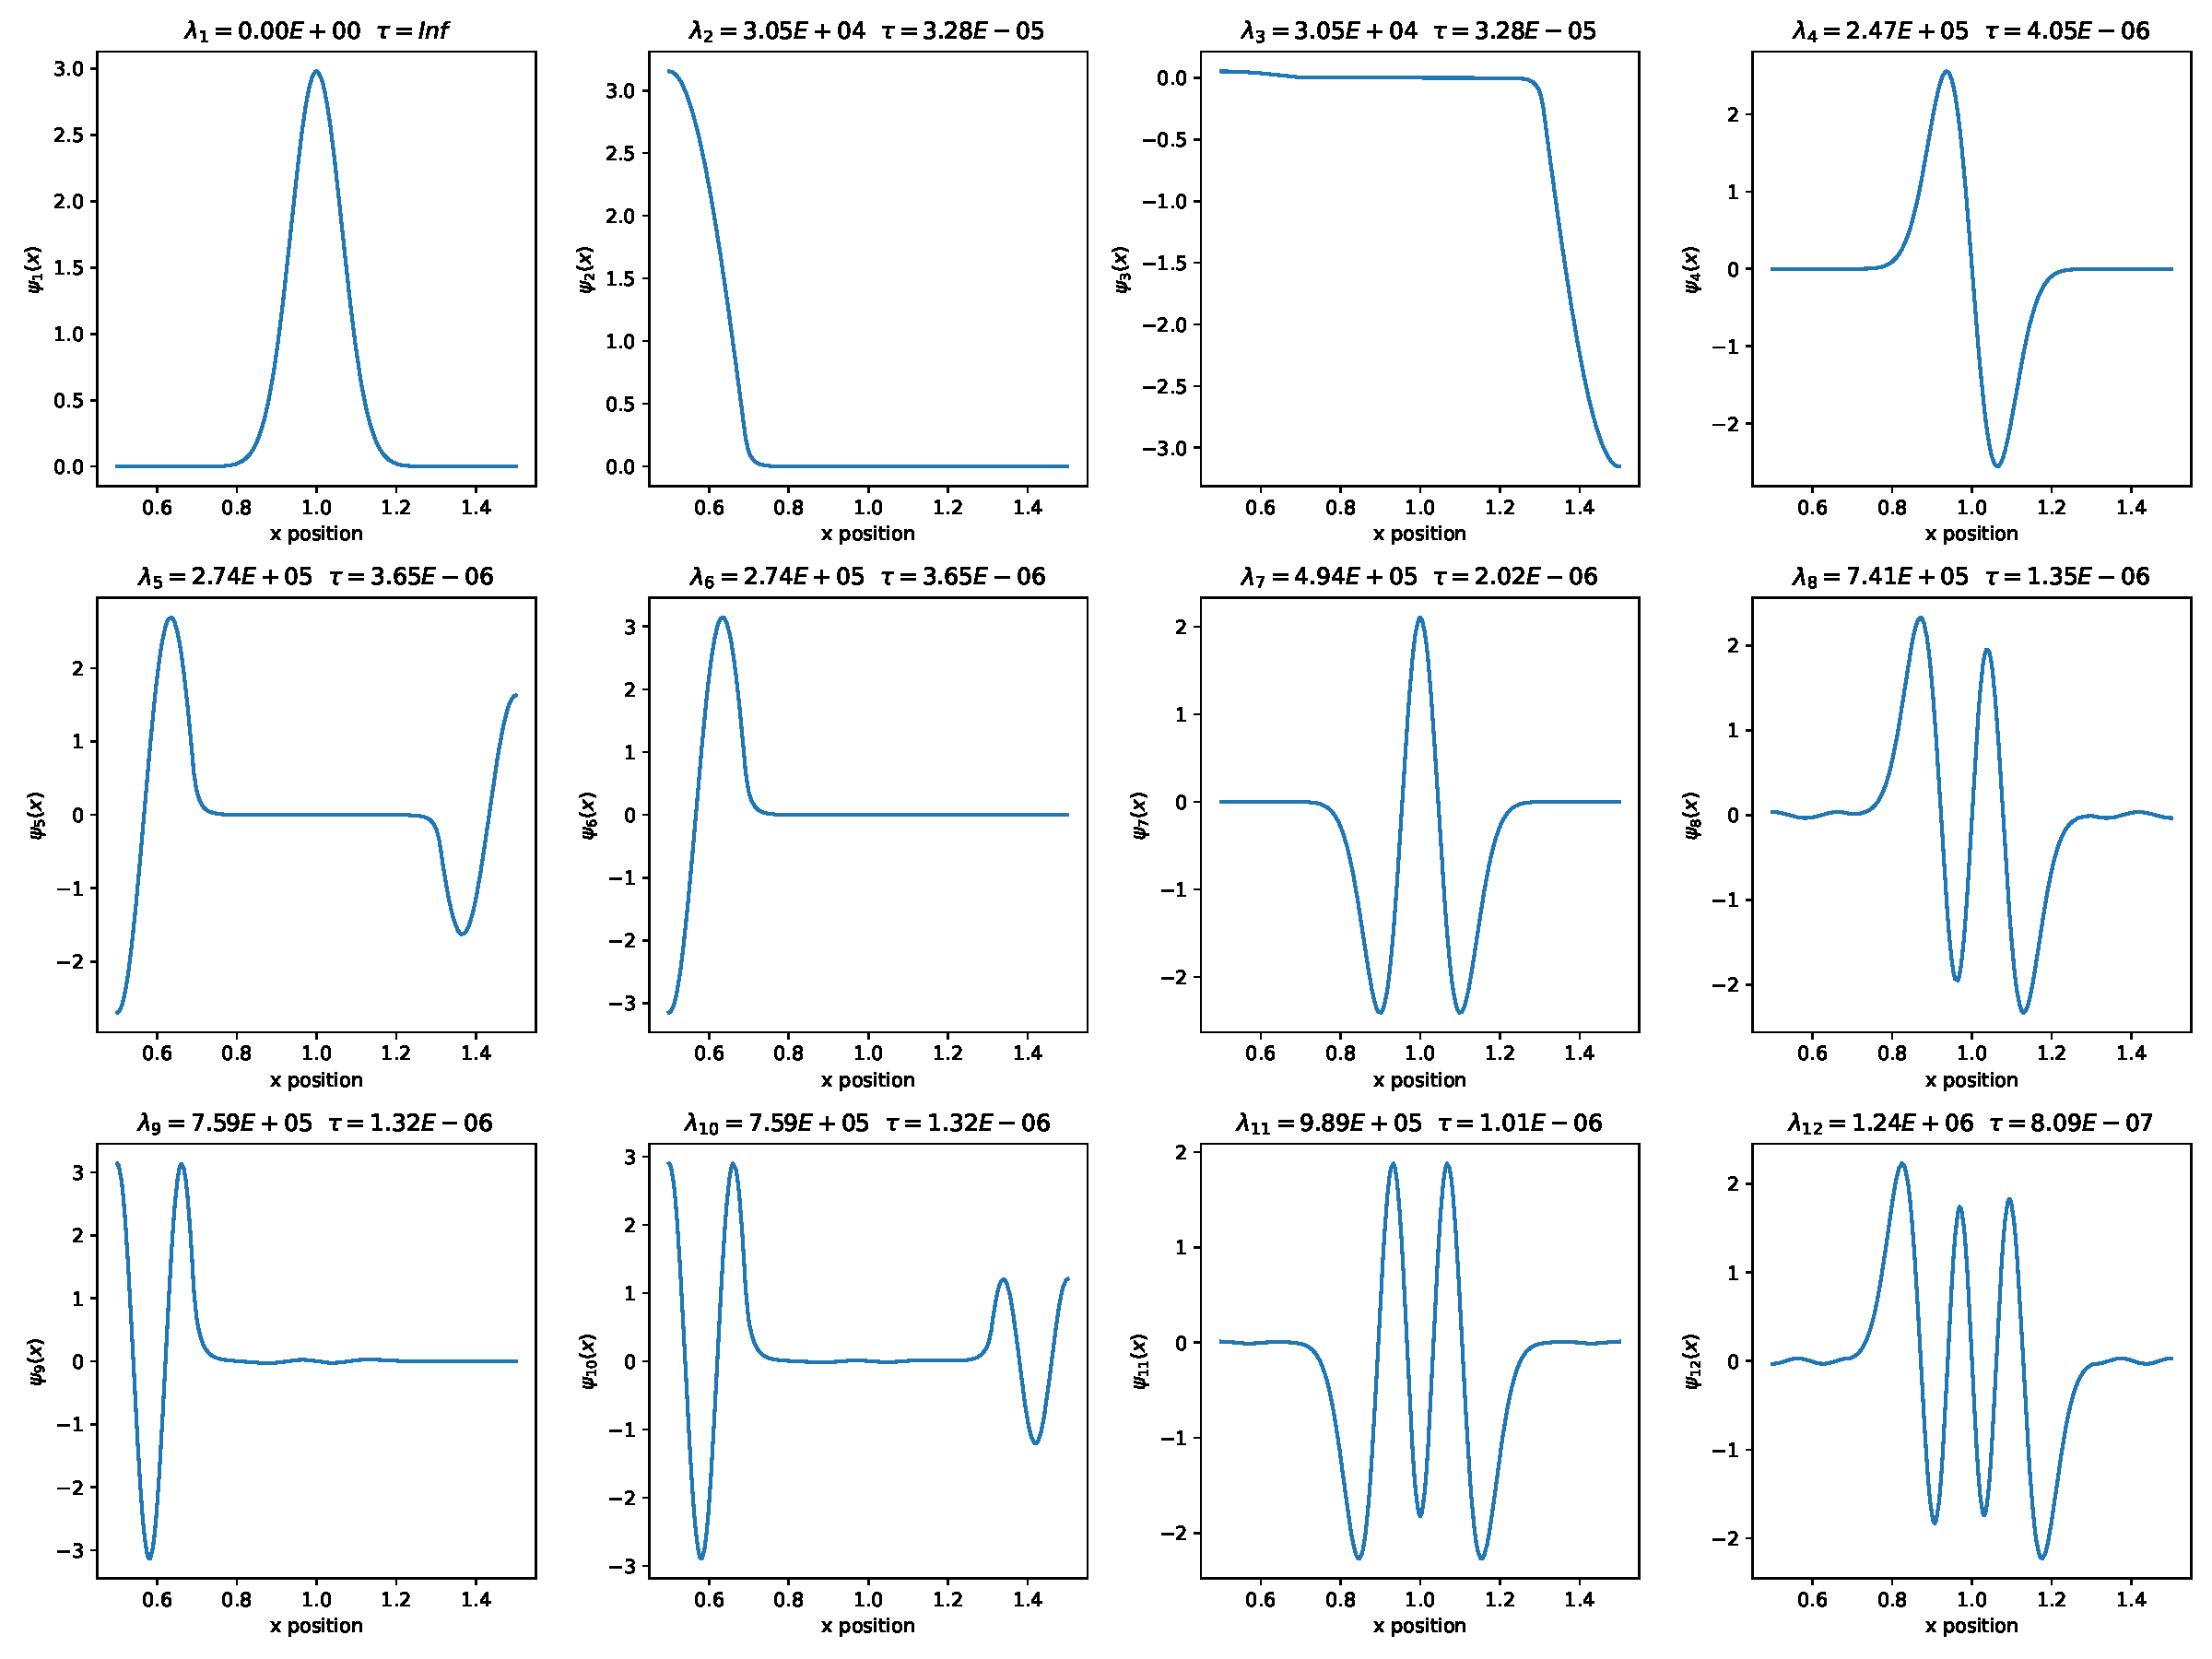
\includegraphics[scale=0.35]{ch3/single_well_2.pdf}   
\end{center}

\section{Double Well}
\begin{center}
        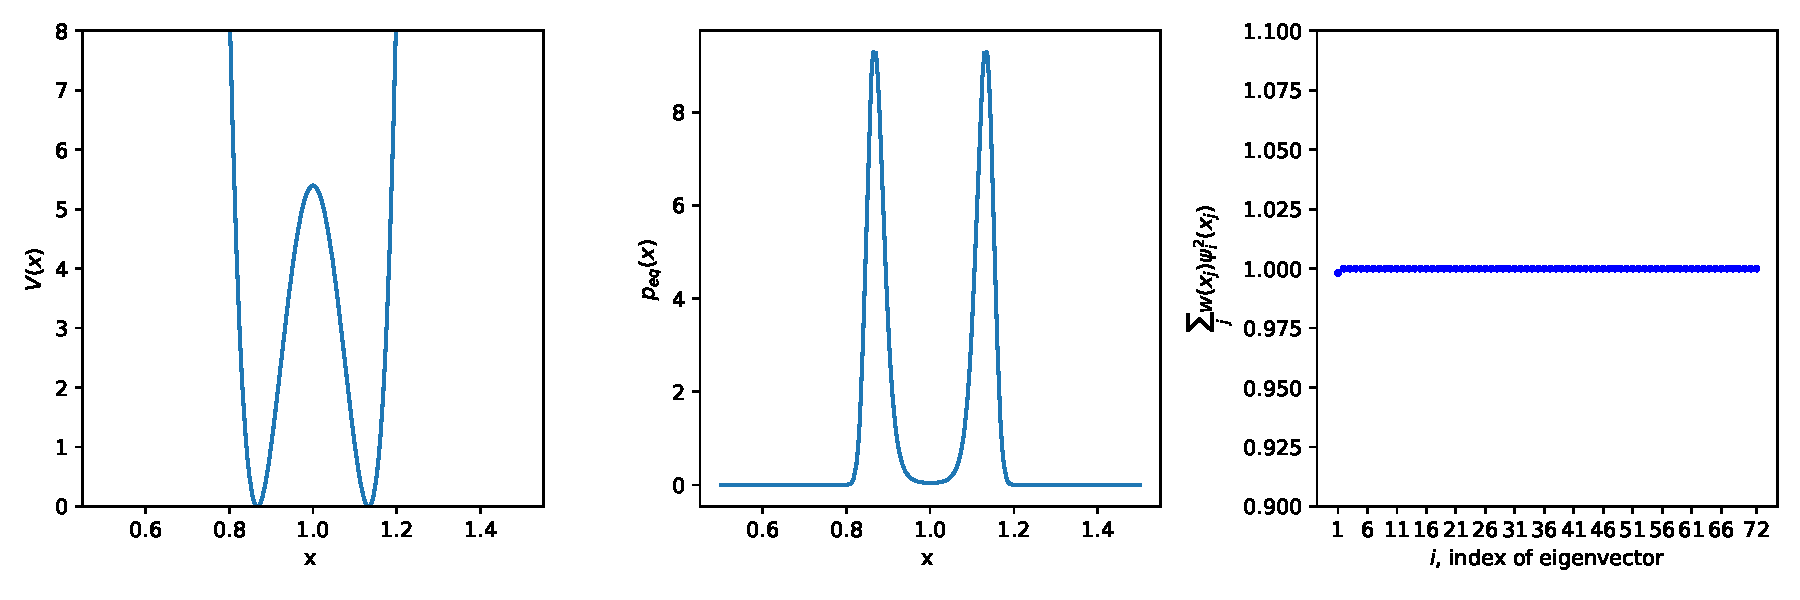
\includegraphics[scale=0.45]{ch3/double_well_1.pdf}   
\end{center}
\begin{center}
        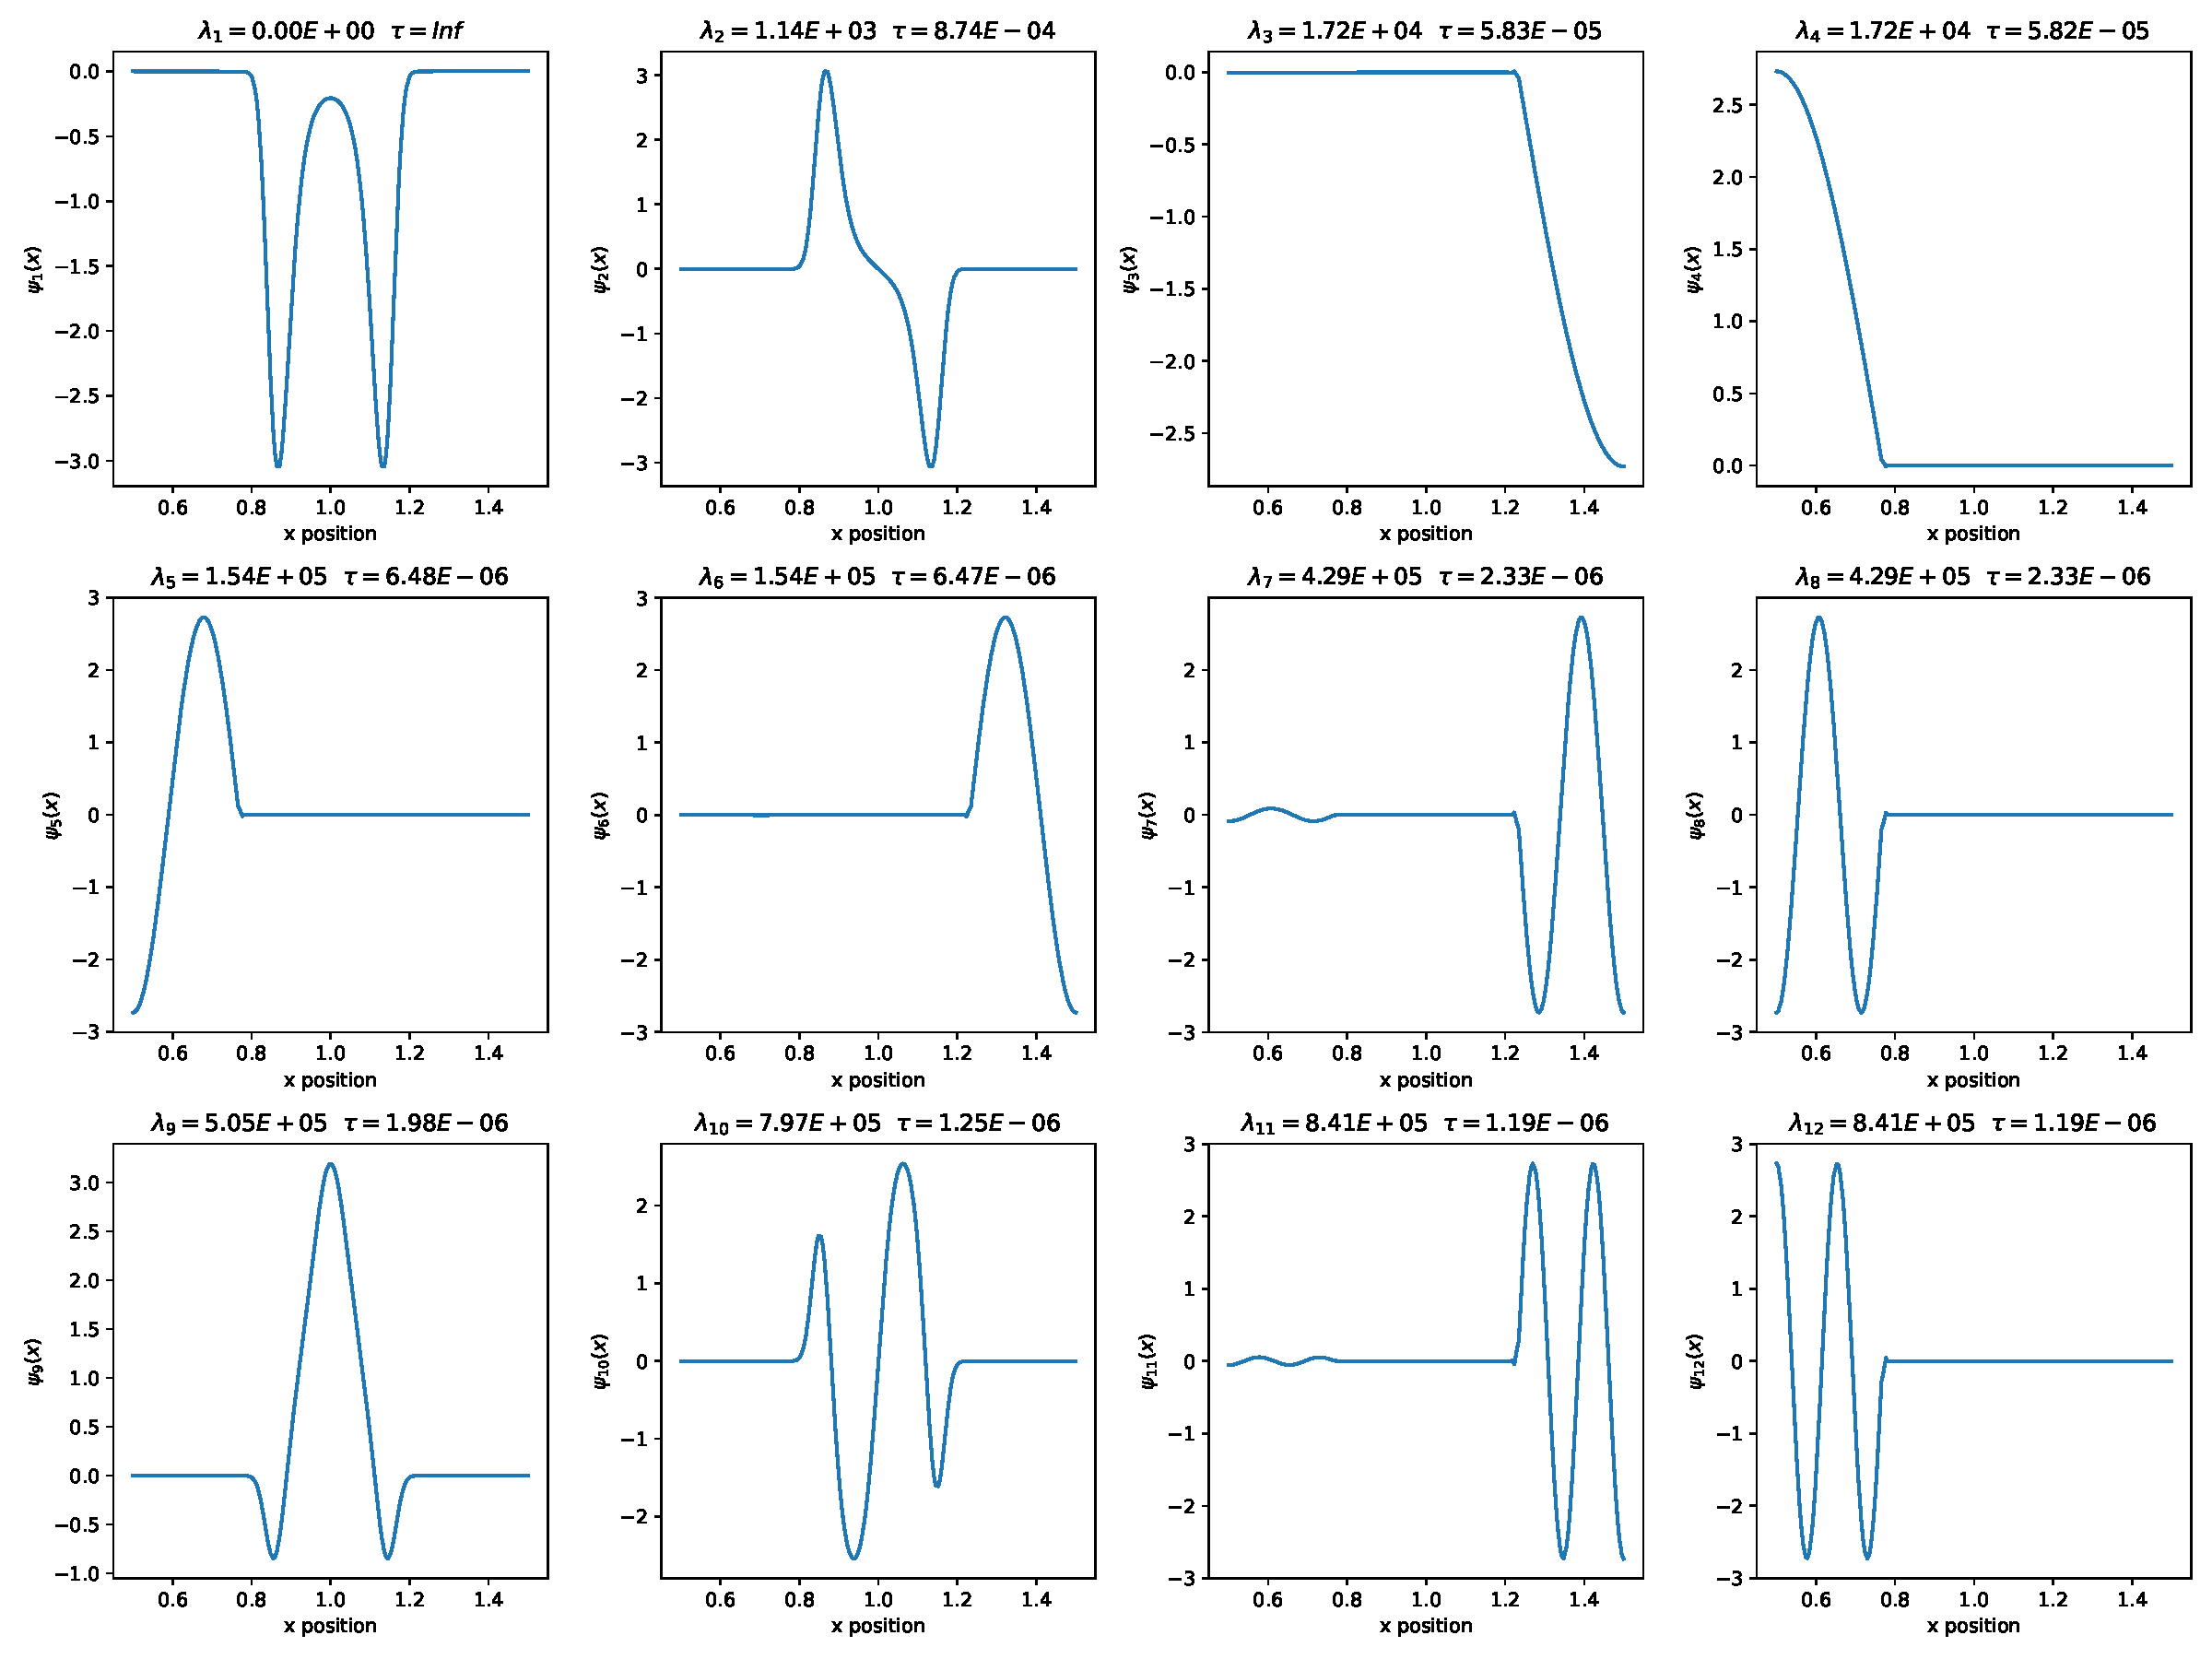
\includegraphics[scale=0.35]{ch3/double_well_2.pdf}   
\end{center}

\section{Triple Well}
\begin{center}
        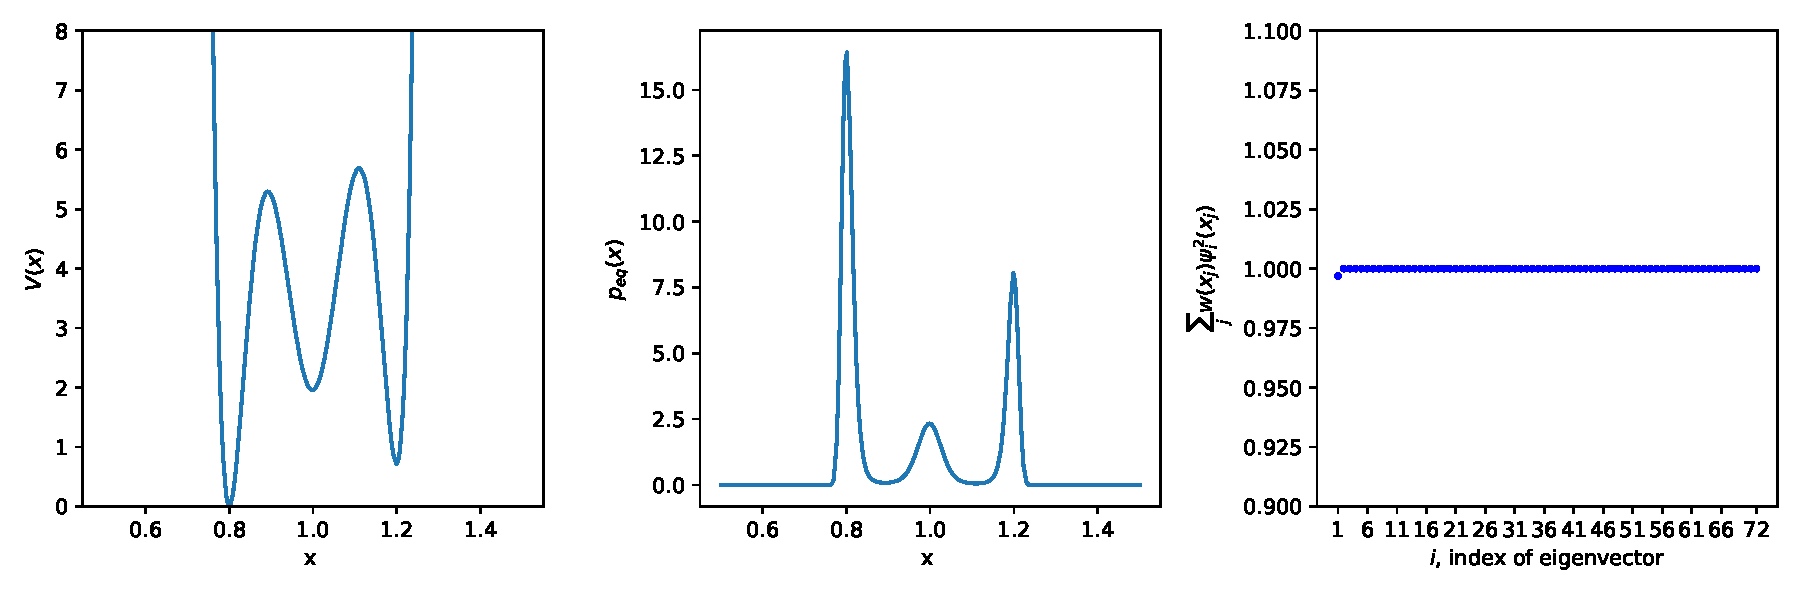
\includegraphics[scale=0.45]{ch3/triple_well_1.pdf}   
\end{center}
\begin{center}
        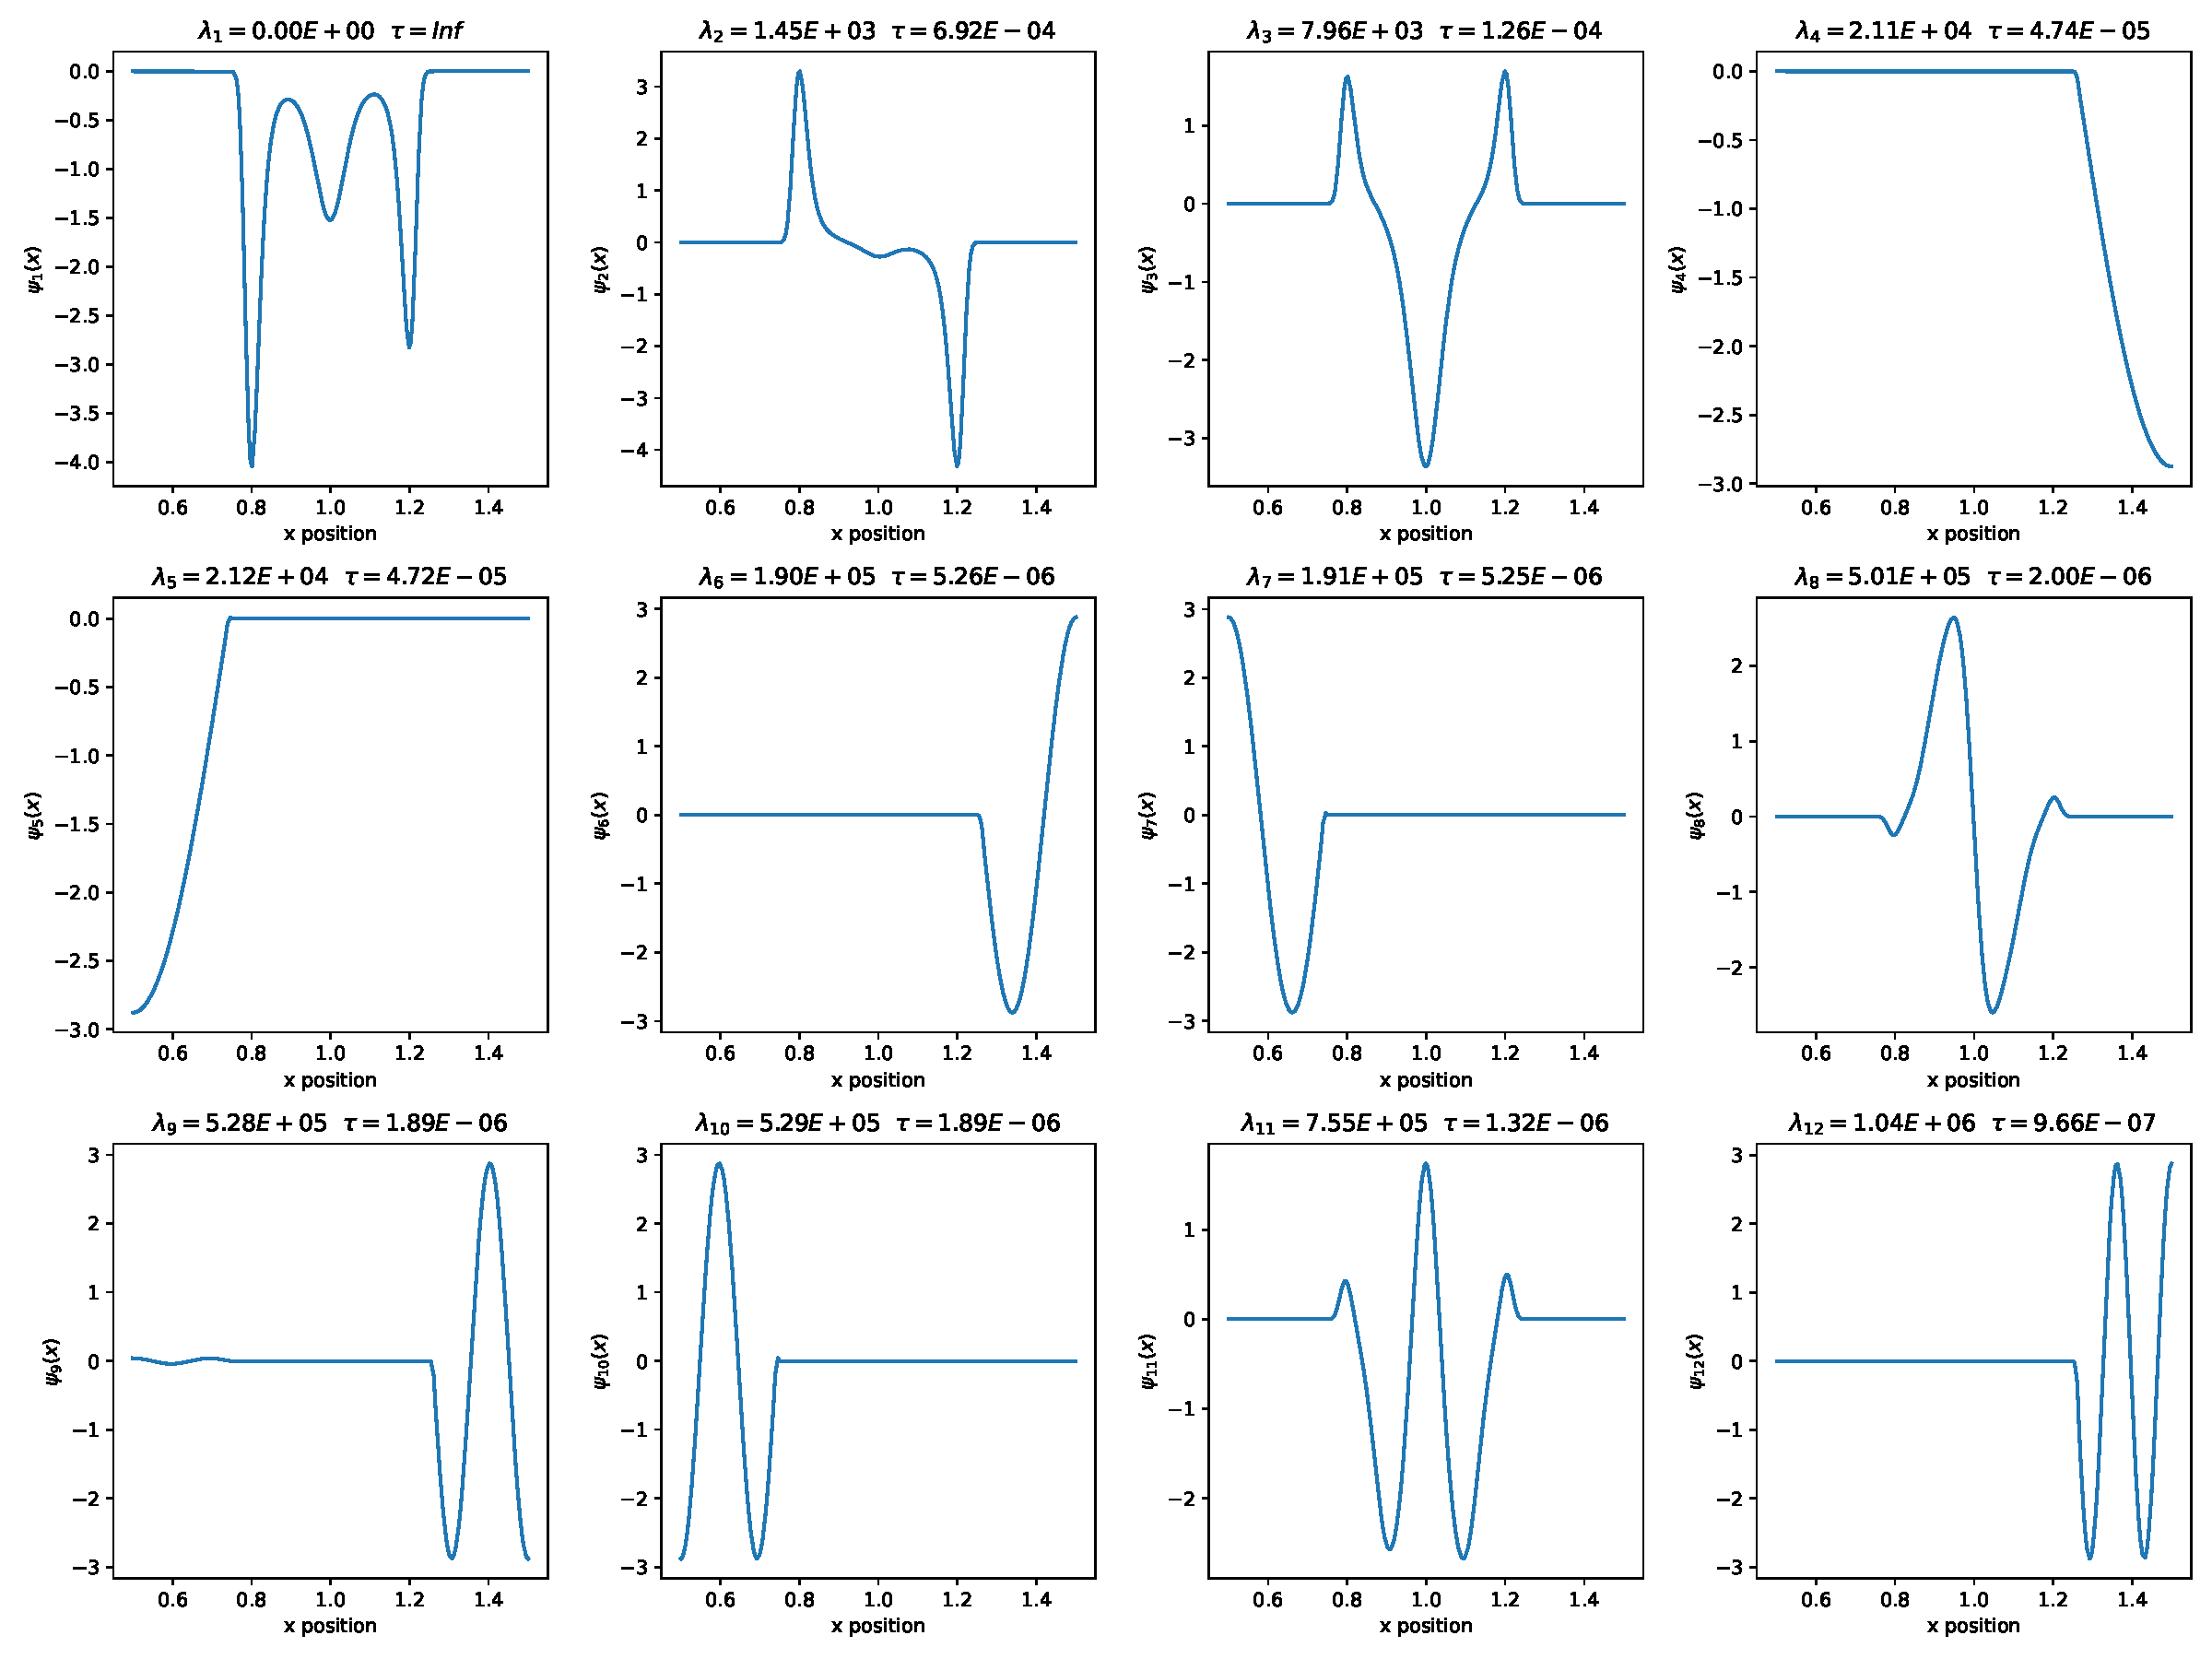
\includegraphics[scale=0.35]{ch3/triple_well_2.pdf}   
\end{center}